\documentclass{beamer}
\usetheme{Warsaw}


\usepackage{lmodern}
%\usefonttheme{structurebold}

\usepackage[francais]{babel}
\usepackage{pgf}
\usepackage[utf8]{inputenc}
\usepackage{latexsym}
\usepackage[T1]{fontenc} 
\usepackage{tikz}
\usepackage{verbatim}
\usepackage{beamerthemeshadow}
\usepackage{caption}
\usepackage{epstopdf}



\AtBeginSection[]{
  \begin{frame}
    \frametitle{Sommaire}
    \tableofcontents[currentsection, hideothersubsections]
  \end{frame}
}

\begin{document}
\title{Soutenance d'EA}
\author{Dhruv SHARMA \\ José MORAN}
\date{25 Février 2016}
\frame{\titlepage}


\section{Introduction}
\begin{frame}{Présentation}
    Lors de cet EA, nous nous sommes intéressés à des méthodes stochastiques de simulation de systèmes quantiques, notamment en utilisant des intégrales de chemin.\pause
    \\    
    $\Rightarrow$ lien entre la physique statistique et la physique quantique à N-corps.
\end{frame}

\begin{frame}{Objectifs}
Simuler des systèmes bosoniques avec des méthodes stochastiques :
    \begin{itemize}
        \item Avec des méthodes de Monte-Carlo diffusif.
        \item Avec des méthodes de Monte-Carlo d'intégrale de chemin.
    \end{itemize}
\end{frame}

\begin{frame}{Plan}
    \begin{itemize}
        \item Présentation des différents outils théoriques.
        \item Présentation des méthodes numériques et de leurs résultats
        \item Le problème des permutations
    \end{itemize}
\end{frame}
\section{Présentation des outils théoriques}
\subsection{Formule de Trotter et fonction de partition}

\begin{frame}{Description du système}
    On se propose d'étudier un système à N corps dans $d$ dimensions décrit par un hamiltonien :
    \begin{equation}
        \hat{H}=\hat{T}+\hat{V}
    \end{equation}
    Où $\hat{V}(x_1,\ldots,x_N)=\sum_{i=1}^N v(x_i)+\sum_{i< j}w(x_i,x_j)$ est la somme d'un potentiel global et d'un potentiel d'interaction entre les particules. 
\end{frame}

\begin{frame}{Fonction de partition}
    Toutes les informations pertinentes sont contenues dans la fonction de partition :
    \begin{equation}
        Z=\mathrm{Tr}(e^{-\beta \hat{H}})
    \end{equation}
    Avec $\beta=\frac{1}{k_B T}$.
    \\
    
    Licite si $\hat{H}$ est borné inférieurement et à résolvante compacte. Dans la pratique :
    \begin{itemize}
        \item Le potentiel global est confinant et le potentiel d'interaction est borné.
        \item On travaille sur un tore
    \end{itemize}
\end{frame}

\begin{frame}{La fonction de partition (suite)}
    $e^{-\beta H}$ est un opérateur à noyau. C'est à dire que : 
    \begin{equation}
        \exists k_\beta, \int_{L\mathbb{T}^d}k_\beta(X,X')\mathrm{d}X'=(e^{-\beta H}\psi)(X)
    \end{equation}
    Ce qui permet d'écrire la fonction de partition :
    \begin{equation}
        Z(\beta)=\mathrm{Tr}\left(e^{-\beta H}\right)=\int k_\beta(X,X)\mathrm{d}X
    \end{equation}
\end{frame}

\begin{frame}{Formule de Trotter}
    On utilise la formule de Trotter :
    \begin{equation}
        (e^{-\beta \hham}\psi)(X)=\lim_{M\to \infty}\left[(e^{-\frac{\beta}{2M}\hat{V}}e^{-\frac{\beta}{M}\hat{T}}e^{-\frac{\beta}{2M}\hat{V}})^M\psi\right](X)
    \end{equation}
    Pour montrer que, à M grand, le système quantique est équivalent à $M$ systèmes classiques intéragissant entre eux, selon un potentiel :
    \begin{multline}
        \mathcal{V}\left(X_0,X_1,\ldots,X_M\right)= \frac{1}{2\beta\sigma^2}\sum_{i=0}^{M-1}|X_{i+1}-X_i|^2\\+\frac{1}{M}\left(\frac{V(X_0)+V(X_1)}{2}+\sum_{i=1}^{M-1} V(X_i)\right)
    \end{multline}
\end{frame}

\begin{frame}{Interprétation comme intégrale de chemin}
On trouve pour $M$ grand : 
    \begin{equation}
        \left(e^{-\beta H}\right) \simeq \frac{1}{(2\pi\sigma^2)^\frac{dNM}{2}}\int_{(\dom)^M} \left(\prod_{i=1}^{M}\mathrm{d}X_i\right) e^{-\beta \mathcal{V}(X,X_1,\ldots,X_M)}\psi(X_1)
    \end{equation}
et on calcule alors :
\begin{equation}
    Z(\beta)\simeq\frac{1}{(2\pi\sigma^2)^\frac{dNM}{2}}\int_{(\dom)^{M}} \mathrm{d}X\left(\prod_{i=2}^{M}\mathrm{d}X_i\right) e^{-\beta S_M(X,X_M,\ldots,X)}
\end{equation}
$\Rightarrow$ interprétation comme une intégrale de chemin.
\end{frame}

\subsection{L'intégrale de chemin}
\begin{frame}{Un outil puissant}
    \begin{itemize}
        \item 
        Outil théorique utilisé generalisant la loi de moindre action pour des systemes quantiques.
        \item 
        S'agit de sommer la contribution des chemins quantiques reliant deux points $x_0$ et $x_n$ à deux instants de temps $t_0$ et $t_n$. 
        \item 
        La correspondance entre l'integrale de chemin et la physique statistique est fait par la fonction de partition. 
        \pause 
        \item 
        L'application numerique se base sur la formule de trotter et l'algorithme de Metropolis.
    \end{itemize}
\end{frame}

\begin{frame}{L'integrale de chemin-suite}
Le terme
    \begin{equation} 
        \label{energie_trotter}
        E = \sum_{j=1}^{M-1}\Big[ \frac{m}{2} \Big( \frac{\mathbf{R}_{j+1} - \mathbf{R}_j}{\Delta \tau}\Big)^2  + V(\mathbf{R}_j) \Big]
    \end{equation}
    
    peut être interpreter comme un terme d'energie potentielle pour un système de $MNd$ particules, ayant des coordonnées $\mathbf{R}_{j}$, pour un système à $N$ particules en $d$ dimensions et à $M$ pas de temps.
    
    \begin{itemize}
        \item 
        Les $Nd$ particules sont couplés entre eux par le potentiel $V$. 
        \item 
        Les particules voisins espacés dans le temps sont couplés par un "ressort" de constant $\frac{m}{\Delta \tau}$. 
    \end{itemize}
\end{frame}


\section{Méthodes probabilistes de simulation}

\subsection{L'algorithme Metropolis}
\begin{frame}{Comment faire du sampling efficace sur des chaînes de Markov ?}
    \begin{itemize}
        \item 
            Construit une chaine de Markov satisfaisant les conditions d'ergodicité et la stationnarité. 
        \item 
            La stationnarité est écrit comme un bilan detaillé 
            \begin{equation}
                \pi(x) P(x \rightarrow x') = \pi(x') P(x' \rightarrow x)
            \end{equation}
            $\pi(x)$ est la distribution stationnaire et $P(x \rightarrow x')$ est la probabilité de passage de l'état $x$ à l'état $x'$ pour la chaine de Markov.
        \item 
            
    \end{itemize}
\end{frame}

\begin{frame}{}
\begin{itemize}
    \item 
    \begin{align} 
        \label{derive_2}
        P(x\rightarrow x') &= g(x\rightarrow x') A(x\rightarrow x') \\
        \frac{A(x\rightarrow x')}{A(x'\rightarrow x)} &= \frac{P(x')}{P(x)}\frac{g(x'\rightarrow x)}{g(x\rightarrow x')}
    \end{align}
    
    \item 
    
    De manière generale, nous choisissons $g(x)$ la distribution uniforme et la probabilité d'acceptation satisfaisant les conditions requises: 
    
    \begin{equation}
        A(x\rightarrow x') = \min\left(1,\frac{P(x')}{P(x)}\right)
    \end{equation}
    
    \item 
    Commode de prendre la probabilité $P(x)$ comme la distribution de Boltzmann: 
    \begin{align} 
        \label{boltzmann_dist}
        P(x) &= \frac{e^{-\beta E_x}}{\mathcal{Z}} 
    \end{align}
\end{itemize}
\end{frame}


\begin{frame}{L'algorithme de Metropolis}
    L'algorithme se déroule de manière suivante: 
    
   \begin{enumerate} 
        \item 
        Nous commençons avec un état $x$
        \item 
        Nous choisissons un nouvel état $x'$ selon la loi uniforme 
        \item 
        Nous acceptons l'état $x'$ selon la loi $A(x\rightarrow x')$. Si l'état est accepté, le nouvel état du système est $x'$. Sinon, le système reste dans l'état $x$ (et donc il n'y a pas de transition)
        \item 
        Nous répétons les étapes 2 et 3 jusqu'à la génération de $\lambda$ états.
    \end{enumerate}
    
\end{frame}
\subsection{Monte-Carlo Diffusif}

\begin{frame}{Description de l'algorithme}
    On fait une marche aléatoire dans notre système, avec le processus défini par : 
    \begin{equation}
        X^{i}_{t+1}=X^{i}_t-\vec{\nabla}V_{tot}(X^{i}_t,X^j_t)+\sigma \sqrt{\Delta t}\xi_t
    \end{equation}
    et on utilise la formule de Feynman-Kac :
    \begin{equation}
        \int_{\Omega} g(x) u(\beta,x) \mathrm{d}x &= \mathbb{E}\left( g(x_{\beta}) e^{-\int_{0}^{\beta} \mathrm{V}(x_s)\mathrm{d}s} \right)
    \end{equation}
    pour calculer des valeurs importantes du système (par exemple l'énergie moyenne)
\end{frame}

\begin{frame}{Potentiel utilisé}
    \begin{figure}
        \centering
        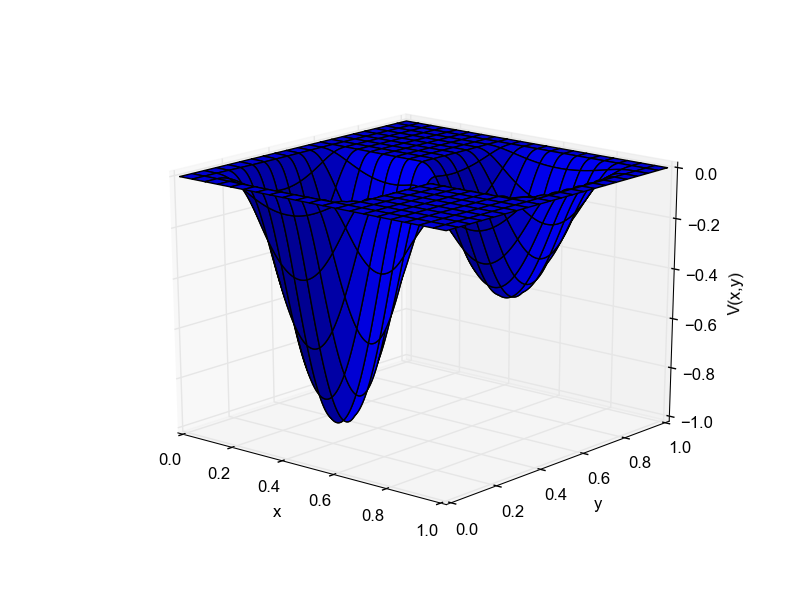
\includegraphics[height=4cm]{Images/potentiel.png}
        \caption{Potentiel utilisé.}
    \end{figure}

\end{frame}

\begin{frame}{Potentiel utilisé}
    Potentiel utilisé : 
    \begin{figure}
        \centering
        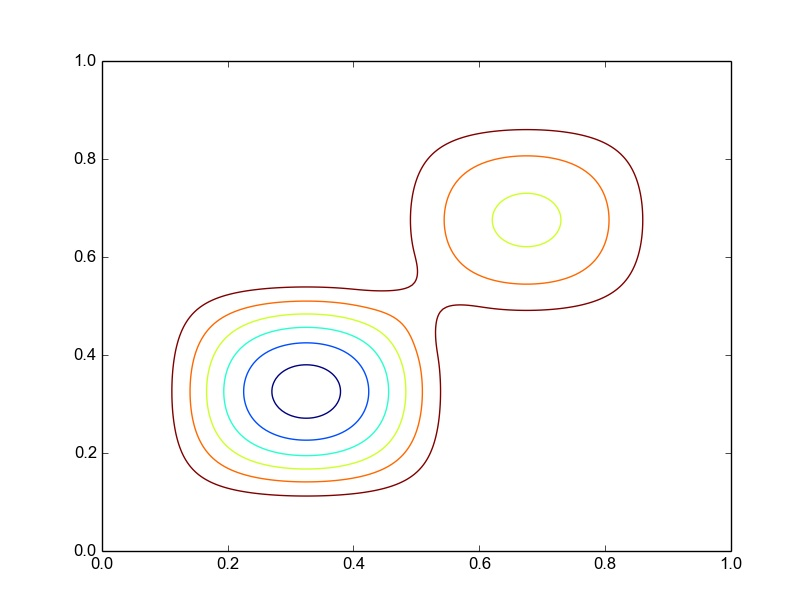
\includegraphics[height=4cm]{Images/potentialiso.jpeg}
        \caption{Lignes de potentiel.}
    \end{figure}
\end{frame}

\begin{frame}{Résultats des simulations}
    \begin{figure}
        \centering
        \includegraphics[height=4cm]{Images/2parts.png}
        \caption{Simulation de deux particules classiques en intéraction entre elles.}
        \end{figure}
\end{frame}

\begin{frame}{Résultats des simulations}
    \begin{figure}
        \centering
        \includegraphics[height=4cm]{Images/energy2parts.png}
        \caption{Energie en fonction de la température}
    \end{figure}
\end{frame}

\begin{frame}{Résultats des simulations}
    \begin{figure}
        \centering
        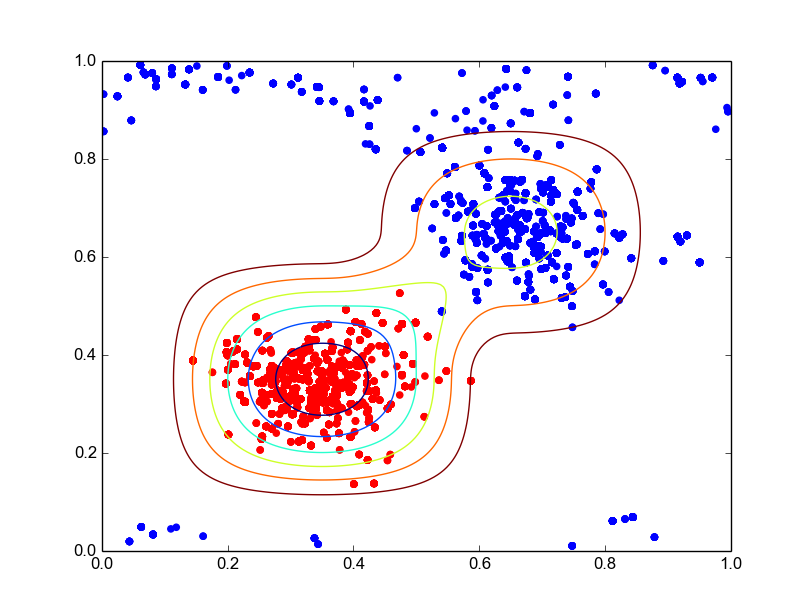
\includegraphics[height=4cm]{Images/quantummc.png}
        \caption{Simulation de deux particules quantiques}
    \end{figure}
\end{frame}

\begin{frame}{Difficultés}
    \begin{itemize}
        \item Taux d'acceptation pour le système classique (2 particules, $10^4$ pas) : $\sim85\%$ 
        \item Temps de calcul pour le système classique : $\sim 20$s. 
        \item Taux d'acceptation pour le système quantique ($M=10$, $10^4$ pas): $\sim 2\%$.
        \item Temps de calcul pour le système quantique : $\sim 3\mathrm{min}$.
    \end{itemize}
\end{frame}
\subsection{Path-Integral Monte-Carlo}

\begin{frame}{Description de l'algorithme}

    \begin{enumerate} 
        \item 
        Nous commençons avec une particule donnée et on fixe deux points $x_0$ et $x_M$. Ici $M$ est le paramètre qui apparaît dans la décomposition de Trotter. Il s'agit de diviser l'axe de temps imaginaire $\beta$ en $M$ tranches. 
        \item 
        Nous initialisons les positions $x_1 \cdots x_{M-1}$ de manière aléatoire. 
        \item 
        Nous choisissons une "tranche" de temps imaginaire $k$ parmi les $M-2$ tranches possibles et on effectue un petit déplacement du chemin d'une distance $dx$. 
        \item 
        Ensuite, nous calculons la différence d'action entre le chemin de départ et le nouveau chemin. 
    \end{enumerate}
    
\end{frame}

\begin{frame}{Resultats}

    \begin{figure}[!h]
        \centering
        % GNUPLOT: LaTeX picture with Postscript
\begingroup
  \makeatletter
  \providecommand\color[2][]{%
    \GenericError{(gnuplot) \space\space\space\@spaces}{%
      Package color not loaded in conjunction with
      terminal option `colourtext'%
    }{See the gnuplot documentation for explanation.%
    }{Either use 'blacktext' in gnuplot or load the package
      color.sty in LaTeX.}%
    \renewcommand\color[2][]{}%
  }%
  \providecommand\includegraphics[2][]{%
    \GenericError{(gnuplot) \space\space\space\@spaces}{%
      Package graphicx or graphics not loaded%
    }{See the gnuplot documentation for explanation.%
    }{The gnuplot epslatex terminal needs graphicx.sty or graphics.sty.}%
    \renewcommand\includegraphics[2][]{}%
  }%
  \providecommand\rotatebox[2]{#2}%
  \@ifundefined{ifGPcolor}{%
    \newif\ifGPcolor
    \GPcolortrue
  }{}%
  \@ifundefined{ifGPblacktext}{%
    \newif\ifGPblacktext
    \GPblacktexttrue
  }{}%
  % define a \g@addto@macro without @ in the name:
  \let\gplgaddtomacro\g@addto@macro
  % define empty templates for all commands taking text:
  \gdef\gplbacktext{}%
  \gdef\gplfronttext{}%
  \makeatother
  \ifGPblacktext
    % no textcolor at all
    \def\colorrgb#1{}%
    \def\colorgray#1{}%
  \else
    % gray or color?
    \ifGPcolor
      \def\colorrgb#1{\color[rgb]{#1}}%
      \def\colorgray#1{\color[gray]{#1}}%
      \expandafter\def\csname LTw\endcsname{\color{white}}%
      \expandafter\def\csname LTb\endcsname{\color{black}}%
      \expandafter\def\csname LTa\endcsname{\color{black}}%
      \expandafter\def\csname LT0\endcsname{\color[rgb]{1,0,0}}%
      \expandafter\def\csname LT1\endcsname{\color[rgb]{0,1,0}}%
      \expandafter\def\csname LT2\endcsname{\color[rgb]{0,0,1}}%
      \expandafter\def\csname LT3\endcsname{\color[rgb]{1,0,1}}%
      \expandafter\def\csname LT4\endcsname{\color[rgb]{0,1,1}}%
      \expandafter\def\csname LT5\endcsname{\color[rgb]{1,1,0}}%
      \expandafter\def\csname LT6\endcsname{\color[rgb]{0,0,0}}%
      \expandafter\def\csname LT7\endcsname{\color[rgb]{1,0.3,0}}%
      \expandafter\def\csname LT8\endcsname{\color[rgb]{0.5,0.5,0.5}}%
    \else
      % gray
      \def\colorrgb#1{\color{black}}%
      \def\colorgray#1{\color[gray]{#1}}%
      \expandafter\def\csname LTw\endcsname{\color{white}}%
      \expandafter\def\csname LTb\endcsname{\color{black}}%
      \expandafter\def\csname LTa\endcsname{\color{black}}%
      \expandafter\def\csname LT0\endcsname{\color{black}}%
      \expandafter\def\csname LT1\endcsname{\color{black}}%
      \expandafter\def\csname LT2\endcsname{\color{black}}%
      \expandafter\def\csname LT3\endcsname{\color{black}}%
      \expandafter\def\csname LT4\endcsname{\color{black}}%
      \expandafter\def\csname LT5\endcsname{\color{black}}%
      \expandafter\def\csname LT6\endcsname{\color{black}}%
      \expandafter\def\csname LT7\endcsname{\color{black}}%
      \expandafter\def\csname LT8\endcsname{\color{black}}%
    \fi
  \fi
  \setlength{\unitlength}{0.0500bp}%
  \begin{picture}(7200.00,5040.00)%
    \gplgaddtomacro\gplbacktext{%
      \csname LTb\endcsname%
      \put(1078,704){\makebox(0,0)[r]{\strut{} 0}}%
      \put(1078,1163){\makebox(0,0)[r]{\strut{} 0.01}}%
      \put(1078,1623){\makebox(0,0)[r]{\strut{} 0.02}}%
      \put(1078,2082){\makebox(0,0)[r]{\strut{} 0.03}}%
      \put(1078,2542){\makebox(0,0)[r]{\strut{} 0.04}}%
      \put(1078,3001){\makebox(0,0)[r]{\strut{} 0.05}}%
      \put(1078,3460){\makebox(0,0)[r]{\strut{} 0.06}}%
      \put(1078,3920){\makebox(0,0)[r]{\strut{} 0.07}}%
      \put(1078,4379){\makebox(0,0)[r]{\strut{} 0.08}}%
      \put(1210,484){\makebox(0,0){\strut{}-4}}%
      \put(1909,484){\makebox(0,0){\strut{}-3}}%
      \put(2608,484){\makebox(0,0){\strut{}-2}}%
      \put(3307,484){\makebox(0,0){\strut{}-1}}%
      \put(4007,484){\makebox(0,0){\strut{} 0}}%
      \put(4706,484){\makebox(0,0){\strut{} 1}}%
      \put(5405,484){\makebox(0,0){\strut{} 2}}%
      \put(6104,484){\makebox(0,0){\strut{} 3}}%
      \put(6803,484){\makebox(0,0){\strut{} 4}}%
      \put(176,2541){\rotatebox{-270}{\makebox(0,0){\strut{}Probability P(x)}}}%
      \put(4006,154){\makebox(0,0){\strut{}Position x}}%
      \put(4006,4709){\makebox(0,0){\strut{}Probability distributions for different values of $\tau$}}%
    }%
    \gplgaddtomacro\gplfronttext{%
      \csname LTb\endcsname%
      \put(5816,4206){\makebox(0,0)[r]{\strut{}$\tau = 0.95$}}%
      \csname LTb\endcsname%
      \put(5816,3986){\makebox(0,0)[r]{\strut{}$\tau = 1.0$}}%
      \csname LTb\endcsname%
      \put(5816,3766){\makebox(0,0)[r]{\strut{}$\tau = 10$}}%
      \csname LTb\endcsname%
      \put(5816,3546){\makebox(0,0)[r]{\strut{}$\tau = 20$}}%
      \csname LTb\endcsname%
      \put(5816,3326){\makebox(0,0)[r]{\strut{}$\tau = 40$}}%
      \csname LTb\endcsname%
      \put(5816,3106){\makebox(0,0)[r]{\strut{}$\tau = 0.50$}}%
      \csname LTb\endcsname%
      \put(5816,2886){\makebox(0,0)[r]{\strut{}$\tau = 100$}}%
      \csname LTb\endcsname%
      \put(5816,2666){\makebox(0,0)[r]{\strut{}$\tau = 1000$}}%
    }%
    \gplbacktext
    \put(0,0){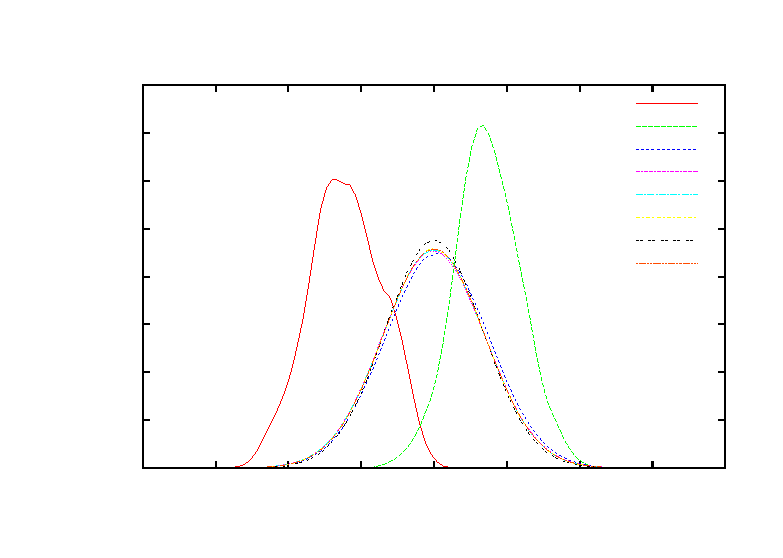
\includegraphics{probability_distributions}}%
    \gplfronttext
  \end{picture}%
\endgroup

        \caption{La distribution de probabilité P(x)}
    \end{figure}
    
\end{frame}

\section{Sampling des permutations}
\subsection{Statistique et mécanique quantique}
    \begin{frame}{Statistique et mécanique quantique}
        Les fonctions d'onde pour les bosons sont symétriques par échange de particules.
        \\
        $\Rightarrow$ il faut symétriser la fonction d'onde en sommant sur toutes les permutations. Il faut donc en tenir compte pour la fonction de partition.
    \end{frame}
\subsection{La difficulté des bosons}
    
\begin{frame}{Permutation des Bosons}
\begin{itemize}
    \item 
    La matrice de densité pour un système à $N$ bosons est écrit comme: 
    \begin{align} 
        \label{densite_boson}
        \rho_{B}( \mathbf{R}, \mathbf{R}'; \beta) = \frac{1}{N!}\sum_{\mathcal{P}} \rho_{\mathrm{D}} (\mathbf{R}, \mathcal{P} \mathbf{R}'; \beta)
    \end{align}
    
    \item 
    Somme sur toutes les permutations $\Rightarrow$ Echantillonnage efficace des permutations aussi.
\end{itemize}
    
\end{frame}



\section{Conclusion}
\end{document}